% Number 750
% SFriction KFriction ETM Algebra Units Vectors
% Pushing crate - angled, friction
% JG

% Watermark
\AddToShipoutPicture*{\BackgroundPic}

\addtocounter {ProbNum} {1}

\begin{floatingfigure}[r]{.22\textwidth}
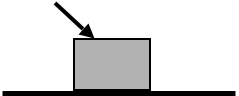
\includegraphics[scale=.6]{/Users/jgates/desktop/latex/pics/pushingbox1}
\end{floatingfigure}
 
{\bf \Large{\arabic{ProbNum}}} A 20 kg crate is pushed along the floor.  Instead of bending down, the worker pushes as shown by the vector, angled downward $40^\circ$. The coefficient of kinetic friction between the crate and floor is .5, and the coefficient of static friction between the crate and the floor is .85.
\bigskip

Determine how much harder (what percentage) the worker will have to push to get the crate moving than if the push was horizontal. \paragraph{}
\noindent
\vfill

\bigskip
Consider the angled push situation and assume that the size of the push is just enough to get the crate moving (and stays constant). Determine the speed of the crate after it has moved 2 meters.
\vfill
%\hfill 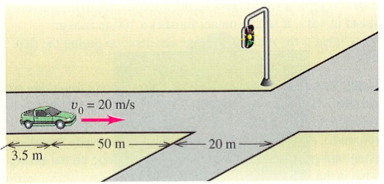
\includegraphics[scale=.85]{/Users/jgates/desktop/latex/pics/redlight.png}
\newpage